\section{THEORETICAL CONCEPTS AND FOUNTATIONS}

This chapter presents brief introductions to the main topics covered in the paper. 
It provides simple and brief background information about the techniques employed here, and serves as a guideline for how all the content has been converged into a single subject.

    \subsection{Convolutional Neural Network}
    Convolutional Neural Networks (CNNs) have been around since the 1940s and their combinations in architectures, are based on biological neural network models capable of recognizing patterns and learning from their interactions with the environment through perception of patterns captured by the senses and processed by equation activated cells, called neurons. 
    In simplest terms, a CNN is a mathematical model performed by a computer, used to process and recognize patterns between inputs and outputs, as a human brain does at each synapse.
    An example of a neural network is shown in Fig.\ref{fig:neura} \cite{LivroNeural}.
    
    \begin{figure}[!h]
        \centering 
        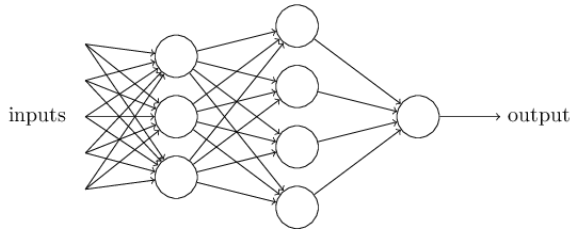
\includegraphics[width=12cm]{Images/cnn.png}
        \caption{Example of three layers CNN. \cite{LivroNeural}}
        \label{fig:neura}
    \end{figure}
    
    In the past few years, merging artificial intelligence technology and computer vision technology have accelerated the search for solutions in many areas.
    Deep learning methods, especially CNNs, reached a state-of-the-art performance and easy to deploy on computer vision, including image classification, features detection, frame to pose estimation, characters recognition, etc. 
    Differently of traditional computer vision approaches, deep learning algorithms doesn't need to be build writing logic of operation, and his design still recognize features and can learn complex representations, increasing his capabilities as the amounts of images in data set also increases.
    
    CNNs are promising tools in a growing number of areas given their versatility to work with data, usually in the form of images, sound, characters, and numbers, or a combination of these elements.
    For this variety of work, neural networks require extensive databases, with many samples of the same type of element to be able to identify it among samples of other elements. 
    This is currently the biggest challenge in much cutting-edge research, since such databases are often, as seen in subsection 3.2, not available in adequate quality, or are not freely available.

    Another issue related to neural networks is that even with an achievable performance for employing their measurements on low-power mobile devices, training the models requires dedicated hardware built for the type of special processing being trained, such as GPUs (Graphics Processing Units) and TPUs (Tensor Processing Units).
    After training, the model consists of a cascade of cells connected in a layer, and these cells have different weights trained by trial and error for successive cycles, called epochs.
    
    
    \subsection{UAV Height Estimation}
    
    The increasing demands of employing UAVs in areas such as security, inspections management and scanning of large areas, transmission lines, and also emergency rescue and natural disasters, demand a lot of effort from the community to get the best out of existing systems, as well as research into innovations for new devices.
    Even with the most modern materials, the fundamentals of height estimation are the same, and are based on reflections. 
    Be it reflections of sound waves, such as ultrasound, or light waves, such as LIDAR or IR \cite{AltitudeEstimationFusion}.
    An example of a UAV with its specific sensors is shown in Figure \ref{fig:sensores}.
    
    \begin{figure}[!h]
        \centering 
        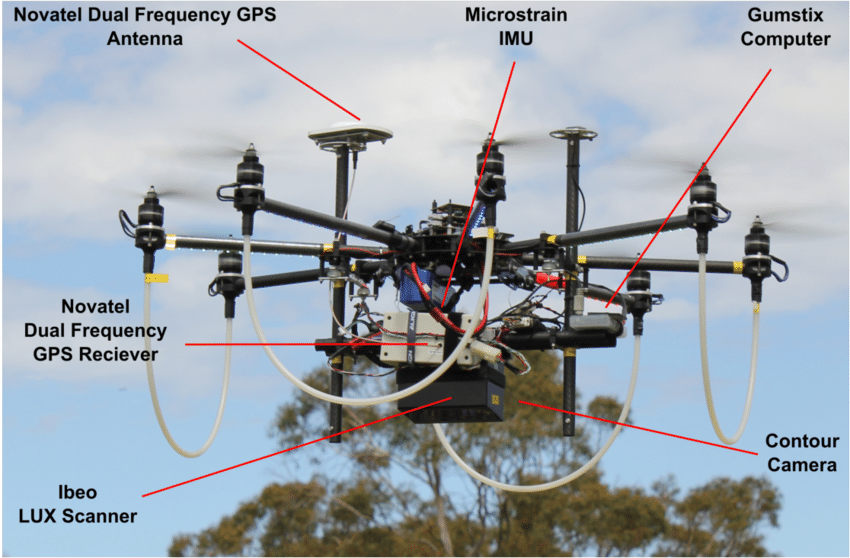
\includegraphics[width=12cm]{Images/sensores.png}
        \caption{Octocopter system with labeled sensors. \cite{SensoresFloresta}}
        \label{fig:sensores}
    \end{figure}
    
    Such signals need to be interpreted by computer systems, to enable decision making, control adjustments, and other deliberations that ensure the desired and safe operation for the vehicle and its surroundings.
    To this end, the efforts of developers of UAV solutions and platforms are divided between computational cost, accuracy, power consumption, physical dimensions, among other concerns concerning a functional system.
    
    Because they are vertical takeoff and landing devices, the use of autopilots in quadcopters and similar devices is impossible without height estimation. Moreover, a good prediction system even helps the operation of human-controlled drones in manual mode, dispensing with the need to correct the climb throttle for hovering.

    One of the most used algorithms capable of performing sensor fusion is the Kalman filter. The Kalman filter is a probabilistic method based on the uncertainties between measurements, and the uncertainties of motion propagated through time, generating a collection of possible results. The input matrices can be composed by measurements of several sensors of the same type, and of different types, thus achieving a great improvement in the accuracy of the system.